 \documentclass[11pt]{report}
  \usepackage{color}
  \usepackage{geometry}
  \usepackage{enumitem}
  \usepackage{mathtools}
  \usepackage{ragged2e}
  \usepackage{listings}
  \usepackage{graphicx}
  \geometry{%
  a4paper,%
  top=2.5cm,%
  bottom=2.5cm,%
  left=2.5cm,%
  right=2.5cm%
}

\begin{document}


\chapter{Cell and their normal functions}
\section{\color{red}Cell as signal analysis device}
\emph{For Biologist :} The cell is the basic structural, functional and biological unit of all known living organisms \cite{wiki:cell}.
\subsection{\color{blue}Cellular Organization}
\subsubsection{Context 1}
Each cell is surrounded by the Extracellular Matrix (ECM) which is a collection of extracellular molecules secreted by the cells that provides structural and biochemical support to the surrounding cells \cite{wiki:ecm}.
Blood cells are such type of cells.
The major structural proteins of the extracellular matrix are members of the large collagen protein family. Collagens form the fibrils that characterize the extracellular matrix of connective tissues, as well as forming networks in basal laminae.

\subsubsection{Context 2}
A group of cells are surrounded by the Extracellular Matrix (ECM).
Skin cells are such type of cells.

\section{\color{red}Concepts of proteins and their role in biological systems}
\subsection{\color{blue}Inside Cells}
\subsubsection{Protein :}
The primary responsibility of proteins is to execute the tasks directed by that information \cite{cooper2007cell}.
Proteins are the most diverse of all macromolecules, and each cell contains several thousand different proteins, which perform a wide variety of functions.
The roles of proteins include serving as structural components of cells and tissues, acting in the transport and storage of small molecules (e.g., the transport of oxygen by hemoglobin), transmitting information between cells (e.g., protein hormones), and providing a defense against infection (e.g., antibodies).
The most fundamental property of proteins, however, is their ability to act as enzymes, which catalyze nearly all the chemical reactions in biological systems.

Ligands and Receptors are also proteins.

Protiens are 'polymers' like molecules which are well structured.
Protiens dictates many aspects of biological systems including signal processing.

Every protein is produced after processing of some gene.
DNA -> RNA -> Protein

\section{\color{red}Level of signal processing in biological cells}
Following are the various levels of signal processing :
\begin{enumerate}
 \item Extracellular level signaling
 \item Cell surface level signaling
 \item Intracellular level signaling
\end{enumerate}

 \chapter{Stem Cells and their role in our body}
 \section{\color{red}Difference between normal cells and stem cells}
 Stem cells differ from normal cells in the following ways \cite{hall1989stem}:
 \begin{itemize}
  \item During the lifespan of an organism, stem cells have unlimited self renewal capacity.
  \item Stem cells can undergo asymmetric cell divisions, i.e., one daughter is itself a stem cell while the other daughter will
  eventually differentiate terminally.
  \item The process of asymmetric division is irreversible as daughters committed to undergo terminal differentiation are not stem
  cells.
 \end{itemize}
 Also the property of \textbf{stemness} allows stem cells to modify their internal signal processing mechanism significantly.
 
 \section{\color{red}The role of stem cells in our body and their working}
 Stem cells are found in many regions of our body like brain, liver \cite{Watt2000}, bone marrow, epidermis, intenstinal epithelium \cite{hall1989stem}, etc..
 Cell divisions have different contributions during embryonic development and during adult life. During embryonic development, cell
 divisions produce new differentiated cells and increase the total number of cells while during adult life, cell divisions maintain the number of differentiated cells
 at a constant level. In tissues with permanently renewing populations like blood, testis, the terminally differentiated cells have
 a very short life span. They are replaced through proliferation of stem cells\cite{hall1989stem}. Stem cells also help in tissue repair by producing
 new cells rapidly.

 \section{\color{red}Life cycle of a stem cell}
 Stem cells have self renewal property and they can either divide Symmetrically or Asymmetrically(Discussed later). A Parent cell
 can either divide into two daughter stem cells or a daughter stem cell and one Transit Amplifying cell Which will eventually differentiate
 terminally.
 
 i.e. 
 
  Parent Cell $\xrightarrow{Symmetric Division}$ [Daughter Stem Cell 1] + [Daughter Stem Cell 2]
  
  \begin{center}
    OR
  \end{center}

  Parent Cell $\xrightarrow{Asymmetric Division}$ [Daughter Stem Cell] + [Transit Amplifying Cell]
  
  \chapter{Differentiation of Stem Cells}
  
  \section{\color{red}Meaning of stem cell differentiation}
  Through the process of cellular differentiation, a less specialized cell turns into a more specialized cell type(Wiki). It can also
  be defined as a qualitative change in the cellular phenotype as a result of the the onset of synthesis of new gene products. A
  cell  can undergo many differentiations during its life. A cell can be differentiated with respect to another cell only as the
  process of differentiation is qualitative\cite{hall1989stem}. For e.g.- A stem cell can differentiate into a brain cell eventually.
  
  
  \section{\color{red}Types of stem cell differentiation}
  There are two types of stem cell differentiation:\\ 
  \begin{enumerate}
   \item \textbf{Natural Pluripotent}: Natural Pluripotent Stem cells have the potential to differentiate into any of the three germ layers: endoderm, mesoderm or ectoderm
   \item \textbf{Induced Pluripotent}: Induced Pluripotent Stem Cells (IPS cells or IPSCs) are a type of Pluripotent stem cells that are artificially derived from non-pluripotent stem cells, by  inducing forced expression of certain genes and transcription factors.

  \end{enumerate}
  
  \chapter{Code structure}
   \section{\color{red} Components of a System}
  The simulation environment consists of the following components:
  \begin{itemize}
   \item Stem Cells
   \item ECM fiber
  \end{itemize}
  
  \section{\color{red} Operations done by simulation class}
  The following operations are supported
  \subsection{\color{blue}Move Cells}
  This function determines the next location for each cell to move to using Gaussian Probability. It calculates the 
  total number of fibers in the neighbourhood and then uses it to calculate probabilty.
  \subsection{\color{blue}Update E Cadherin - $ \beta $ Catenin value}
  This function updates the E Cadherin - $ \beta $ Catenin value based on the following logic:
  \begin{itemize}
   \item Calculate the total ECadherin value by summing the ECadherin value of all the neighbours.
   \item Use the following formula to update the ECadherin- $\beta$ Catenin value:\\
   \begin{equation}
    EB = \frac{sumFiber}{sumFiber+k} + \frac{totalNeigbourEC}{N}
   \end{equation}
   where
   \begin{description}[labelindent=2cm]
    \item \textbf{sumFiber} = The sum of the fiber counts of the neighbours
    \item \textbf{k} = A constant
    \item \textbf{totalNeighbourEC} = total E Cadherin value
    \item \textbf{N} = Number of neighbours
    \end{description}
   \end{itemize}
   \subsection{\color{blue}Evolve genetic code}
   Changes the genetic code array as
   \begin{itemize}
    \item geneticCode[0]=geneticCode[0] AND geneticCode[1]
    \item geneticCode[1]=geneticCode[1] OR geneticCode[2]
    \item geneticCode[2]=NOT geneticCode[2]
   \end{itemize}

  \subsection{\color{blue}Increase age of cells}
  This function increases the age of all cells by 1 and splits(divides) a cell into two if its age becomes more than 30.
  The location of the new cell is determined using Gaussian probabilty concept as used in moving cells.

  \section{\color{red} Operations done by cell class}
  The following operations are supported
  \subsection{\color{blue}Increase cell age}
  This function increases the age of cell by 1.
  
  \section{\color{red} Operations done by AutomatonCell class}
  The following operations are supported
  \subsection{\color{blue}Increase number of fibers at that point}
  This function increases number of fibers at that particular point by 1.
  
  \section{\color{red} Operations done by Utilities class}
  The following operations are supported
  \subsection{\color{blue}Generate output ECM file}
  This function writes the state of lattice (Environment) in file "ptMap.xyz" in following format : \\
  \begin{itemize}
    \item First line specifies the number of points in the xyz file.
    \item Second line is a comment line
    \item Remaining lines specifies each point (record) in format : \\
    $<cell Type> <x Dimension> <y Dimension> <z Dimension> <cell Count>$
   \end{itemize}
   \subsection{\color{blue}Write current state/iteration}
   This function writes the state/iteration changes of lattice (Environment) in a file named "$<iterationNumber>$.txt" in the following format :
   \begin{itemize}
    \item For each point in the lattice, following values are specified \\
    $<x Dimension>,<y Dimension>,<z Dimension>,<cell Type>,<cell Id>,<cell Age>$ \\ \\
    Note : cell age is -1 for empty (free) points 
   \end{itemize}
  
  \chapter{Implementation}
  \section{\color{red}Classes}
  \subsection{\color{blue}AutomatonCell}
  \paragraph{Description}
  Class representing a Lattice Point
  \subsection{\color{blue}Cell}
  \paragraph{Description}
  Class representing a cell
  \subsection{\color{blue}Environment}
  \paragraph{Description}
  This class provides functions for setting up the simulation environment
  \subsection{\color{blue}Line}
  \paragraph{Description}
  Class representing a line in 3d plane
  \subsection{\color{blue}Point}
  \paragraph{Description}
  Class representing a 3 dimensional point
  \subsection{\color{blue}Simulation}
  \paragraph{Description}
  This class provides necessary functions for performing the simulation
  \subsection{\color{blue}SimulationParameters}
  \paragraph{Description}
  Class for loading simulation parameters
  \subsection{\color{blue}StemCell}
  \paragraph{Description}
  This class models the Stem Cells and is derived from the Cell class
  \subsection{\color{blue}TACell}
  \paragraph{Description}
  This class models the Transit Amplifying Cells and is derived from the Cell class
  \subsection{\color{blue}Utilities}
  \paragraph{Description}
  Class for generating the Output
  \subsection{\color{blue}Var}
  \paragraph{Description}
  Class representing a coordinate variable
  \pagebreak
  \section{\color{red}Class Diagram}
    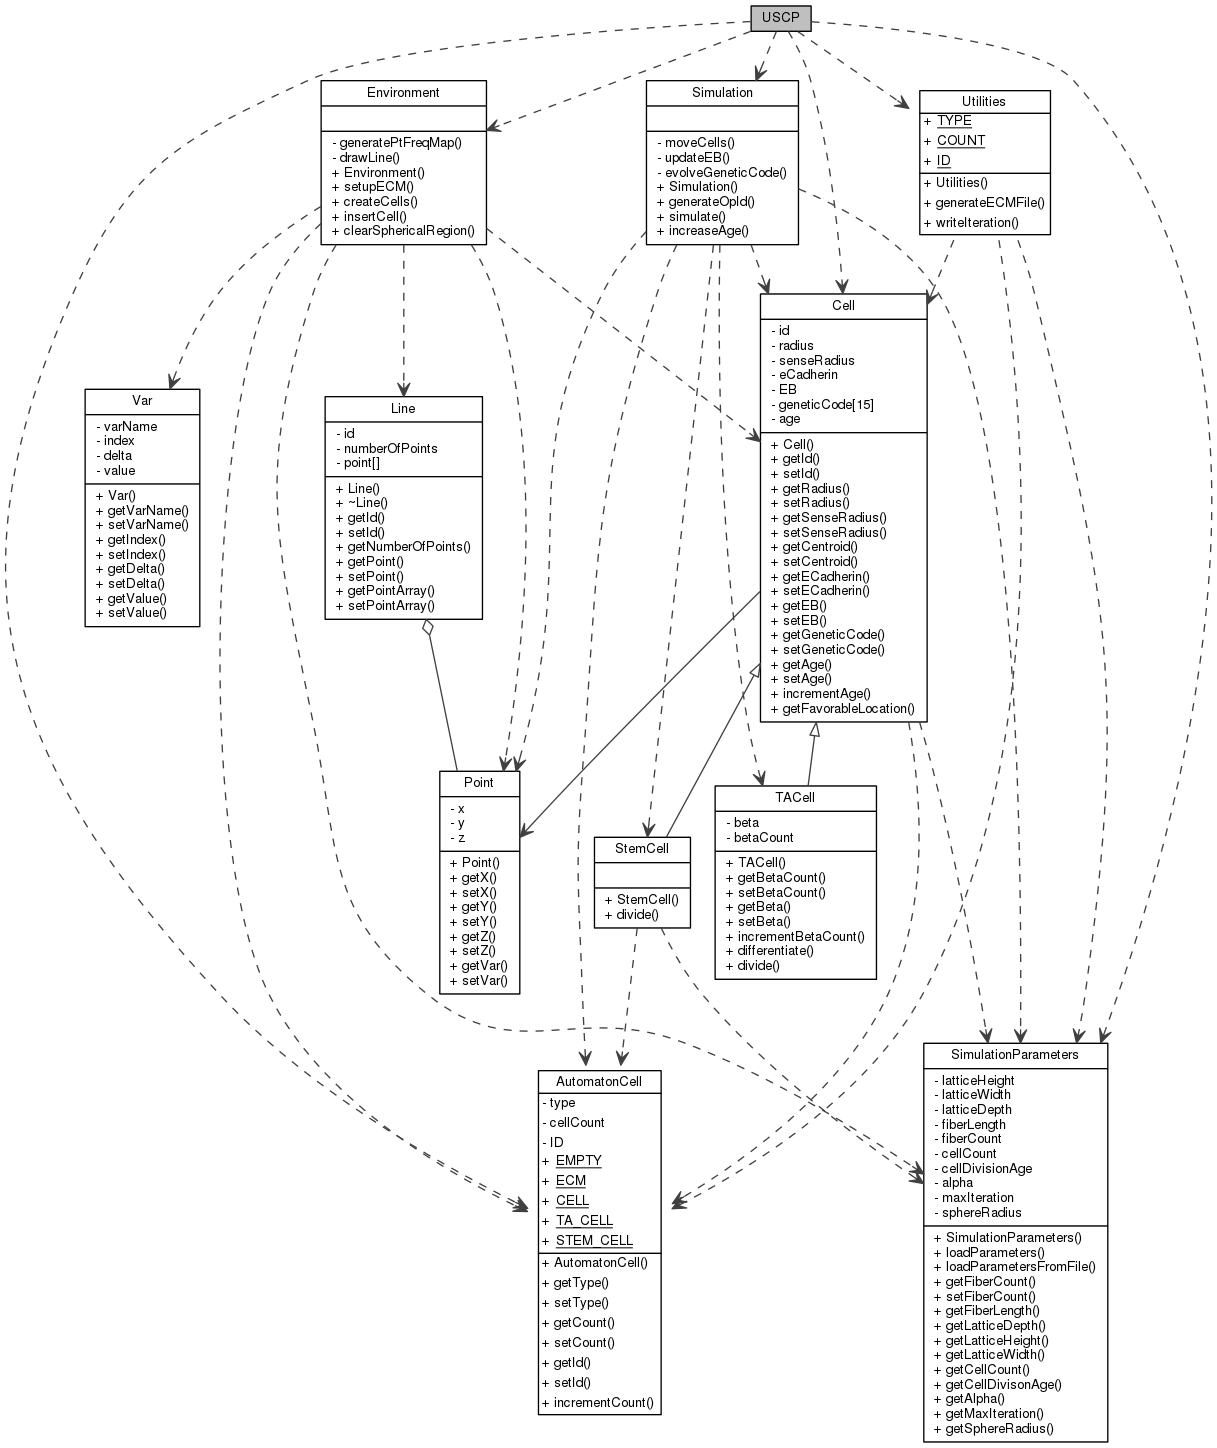
\includegraphics[width=7in]{../diag/classDiagram/class_diag.png}
  
  \section{\color{red}Description of Configuration Files}
  \subsection{\color{blue}"uscp.conf"}
  \subsubsection{\color{green}Description: }
  The structure of uscp.conf is as follows:
  \begin{itemize}
   \item \textbf{Parameters} : The root of xml file.
   \begin{itemize}
    \item \textbf{Lattice} : Represents the simulation environment.
    \begin{itemize}
     \item \textbf{Height} : The Height of the lattice.
     \item \textbf{Width} : The Width of the lattice.
     \item \textbf{Depth} : The Depth of the lattice.
    \end{itemize}

    \item \textbf{FiberCount}: The number of fibres in the lattice.
    \item \textbf{FiberLength} : The Length of each fibre.
    \item \textbf{CellCount} : The number of normal cells present at the beginning of simulation.
    \item \textbf{CellDivisionAge} : The age after which the cell divides.
    \item \textbf{Alpha} : The probability of asymmetric division of stem cells.
    \item \textbf{MaxIteration} : The maximum number of simulation iterations.

   \end{itemize}

  \end{itemize}
  
  \subsubsection{\color{green}Code: }
  \lstset{language=XML}
  \lstinputlisting{../../uscp.conf}


  
 \bibliographystyle{plain}
 \bibliography{StemCellsReferences}
\end{document}
